\hypertarget{la-chine-au-pas-de-course}{%
\section{La Chine au pas de course}\label{la-chine-au-pas-de-course}}

\emph{Samedi 16 juin 2018}

Depuis notre arrivée en Chine, le rythme de notre voyage s'est accéléré.
Après avoir passé deux semaines pour visiter deux villes en Russie, la
cadence de deux jours par ville est un peu rude ! Les étapes de notre
parcours jusqu'ici ont été : Shanghai, Suzhou, Beijing, Gubeikou, Xi'an.

Après nos deux premières nuits à Shanghaï, marquées surtout par une très
mauvaise tolérance du décalage horaire surajouté à la nuit blanche du
voyage (on vous a pas raconté la correspondance ratée, mais elle a été
marquée par une scène mythique de course à travers l'aéroport de Wuhan
avec nos sac à dos, derrière l'employé de la compagnie qui arrêtait pas
de crier "hurry up! hurry up!", alors que bon les 3 heures de retard de
notre vol, on les avait pas vraiment demandées...), on a pris un train
pour notre première étape : Suzhou.

Première expérience de train, un peu effrayante (surtout qu'on venait
d'acheter pour 200 euros de billets de train à travers le pays) : ce
sont des trains type TER, donc pas très rapides et faisant de nombreux
arrêts, d'allure plutôt vétuste. Il y a 5 sièges par rangée, face à
face, dont l'assise fait à peine plus que la moitié des assises
auxquelles ont est habitués. Les tout petits porte-bagages sont pris
d'assaut par les sacs de courses des gens qui rentrent en banlieue
(c'est pas l'Essonne hein, on parle d'un tout autre ordre de
grandeur...) et le train est complètement surbooké, avec des gens debout
dans tous les sens. Les contrôleurs jouent à se chamailler entre eux,
les gens se pressent au distributeur d'eau chaude pour manger leur boite
de nouilles instantanées ou juste remplir leur gourde à thé qu'ils ne
lâchent pas. Bon, on va dire que pour une heure de train, ça se fait
plutôt bien, et puis c'est un peu une "expérience d'un autre âge" (clin
d'oeil à Ruocong).

\begin{figure}
\centering
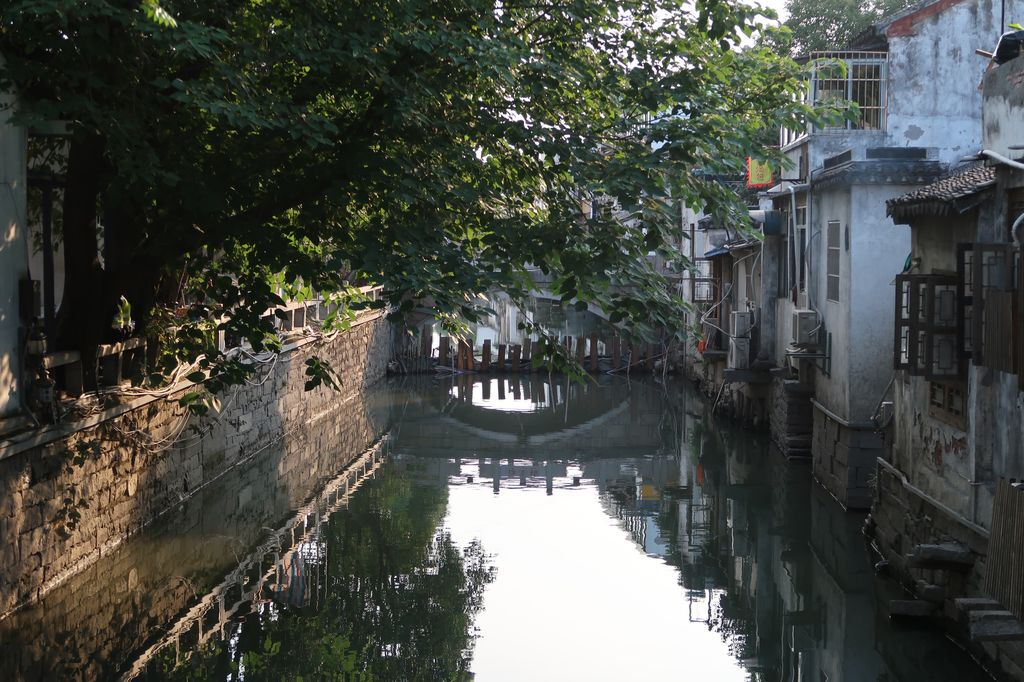
\includegraphics{images/20180616_suzhou.JPG}
\caption{L'un des canaux du vieux centre de Suzhou.}
\end{figure}

Faut dire qu'après ça, on était bien contents de prendre un taxi pour
rejoindre notre auberge, sur le canal central de la ville. Oui parce que
Suzhou, c'est "la Venise de l'Orient", une ville dont le centre est
quadrillé par des canaux et ponctuée par des jardins traditionnels aux
noms rigolos dispersés à ses quatre coins. Les balades au fil de l'eau
étaient plutôt agréables, mais l'agrément des jardins était vite altéré
par les hordes de touristes à perche (à selfie). Le meilleur moment de
notre court séjour a été la visite d'un temple bouddhiste, un peu à
l'écart. On a été accueillis par une statue de Bouddha souriant devant
une belle pagode, mais aussi par une dame qui travaille dans le temple
et qui a appris à Elida à prier en chinois, puis par un maître
calligraphe qui nous a appris à écrire "France" sur le sol du temple,
puis par un moine bouddhiste qui nous a offert des délicieux fruits dont
on n'a toujours pas réussi à retenir le nom, puis par un monsieur de
Pékin qui se prélassait sur un promontoire et qui a discuté avec nous
pendant que nous sortions ensemble du temple. Un vrai moment de calme et
de générosité...

Mais le calme est de courte durée, nous avons un train de nuit à
attraper pour notre troisième étape : Pékin !

Deuxième expérience de train, que nous abordons avec méfiance, surtout
qu'il s'agit de rester 11 heures dans le machin. C'est finalement une
très agréable surprise, car les trains de la ligne Shanghaï-Pékin ont
été récemment remplacés par des trains-couchette extrêmement
confortables et bien équipés. D'après Flo, grand habitué des voyages
nocturnes : "c'est le meilleur train de nuit de toute ma vie !", et on
était qu'en deuxième classe !

\begin{figure}
\centering
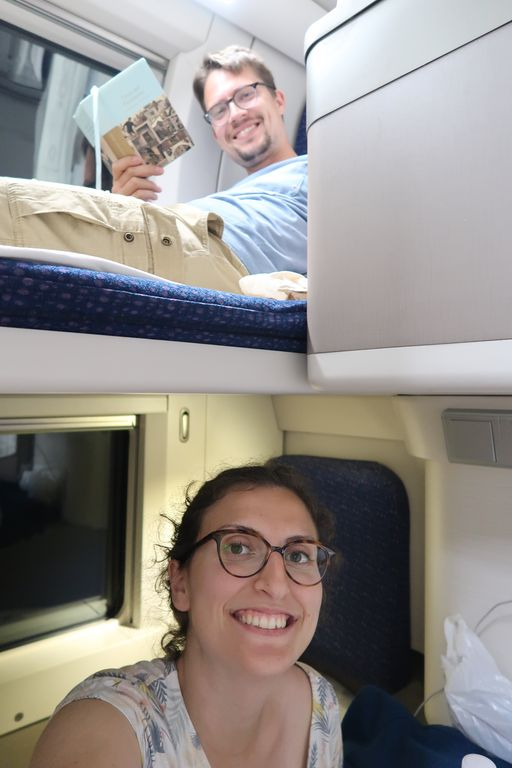
\includegraphics{images/20180616_trainnuit.JPG}
\caption{Selfie dans le train de nuit D312. Flo est en train de lire
Dostoïevski, souvenir emporté de Russie.}
\end{figure}

Nos premiers pas à Pékin nous propulsent un peu plus loin dans le
dépaysement. Notre auberge, le Red Lantern (coucou les Thibali ! on a vu
\emph{a posteriori} que vous y êtes passés aussi !) se trouve dans un
\emph{hutong}, un de ces quartiers typiques de la ville constitués de
ruelles et de petites maisons basses. Et comme on est levés tôt, on
commence la journée par la visite de la Cité Interdite ! Cet
enchaînement de palais en enfilade qui se termine par un jardin nous
fait voyager plus de 500 ans en arrière... et le flot dense de touristes
nous ramène à la réalité, et rend la visite vite pénible (80 000
touristes par jour, c'est 1 fois et demi Disneyland Paris en plein été).
Voilà que l'orage s'en mêle et on s'abrite dans les petits palais
latéraux où sont exposés des objets des différentes dynasties. Le temps
que la météo se calme, on est devenus experts en céramique chinoise ;)
On continue la journée par une balade depuis les "Drum Tower" et "Bell
Tower", anciennes tours jumelles qu'on retrouvera en fait dans toutes
les vieilles villes du pays, puis par le parc Beihai et le parc Jingshan
depuis lequel on a une vue panoramique sur la Cité Interdite et sur un
beau coucher de soleil sur Pékin.

\begin{figure}
\centering
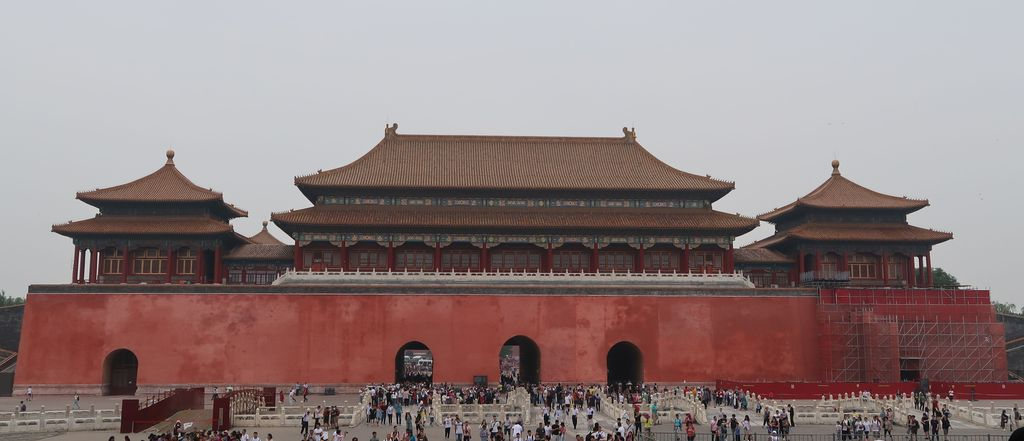
\includegraphics{images/20180616_cite.JPG}
\caption{L'un des palais de l'Harmonie de la Cité Interdite}
\end{figure}

La visite du Palais d'Eté le lendemain nous permettra de nous échapper
de la chaleur étouffante de la ville. On se s'attarde pas sur les
bâtiments, mais la visite est tout de même intéressante. Le tour du lac
nous permet de nous écarter des foules, ce qui est toujours très
agréable ! Le soir, sur des recommandations expertes, nos papilles
découvrent le vrai canard à la pékinoise, grillé à point et découpé avec
art sous nos yeux. Nous qui étions soucieux de ne pas pouvoir finir un
canard entier, nous l'avons dévoré jusqu'à la dernière miette !

\begin{figure}
\centering
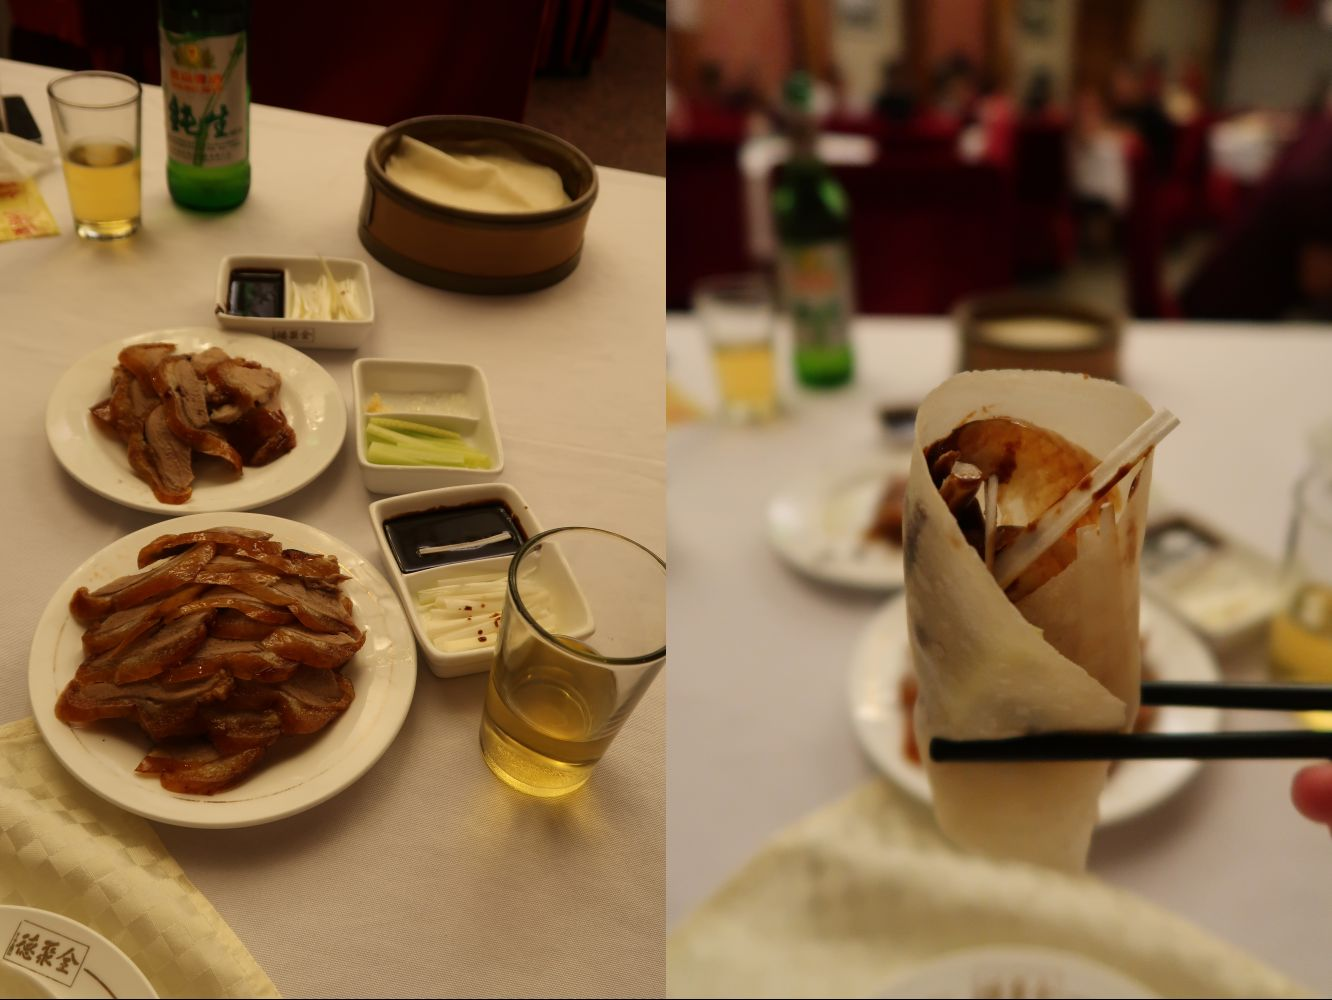
\includegraphics{images/20180616_canard.jpg}
\caption{Avant / après : voici comment on nous a appris à manger le
canard de Pékin.}
\end{figure}

Nous avons fait nos derniers pas à Pékin au temple des Lamas, constitué
de plusieurs bâtiments successifs dont la magnificence va crescendo
jusqu'au dernier où trône une statue de Bouddha debout de 18 mètres de
haut taillé dans une seule pièce de bois. Après avoir avalé un délicieux
Jianbing (une sorte de crêpe salée à l'oeuf et au sésame, garnie de
salade, d'oignon vert, de sauces diverses et de tofu grillé), on part
pour un périple en bus qui nous prendra 4 heures pour une destination
reculée : Gubeikou.

A Gubeikou nous attend Angela, notre hôte, avec un délicieux repas à
base de légumes de son potager, mais surtout la grande muraille de Chine
! Quelques dizaines de minutes de marche et la muraille est sous nos
pieds, d'aspect brut, sans rénovation. Il semble incroyable qu'on ait pu
construire un tel édifice... Comme on a fait l'effort de se lever tôt,
on passe près de 2 heures complètement seuls sur la muraille, entourés
de nombreux oiseaux, dans l'air frais du matin. L'expérience est unique,
la muraille s'étend à perte de vue des deux côtés au milieu d'une forêt
luxuriante, et même sur le flanc raide d'une montagne au loin.

\begin{figure}
\centering
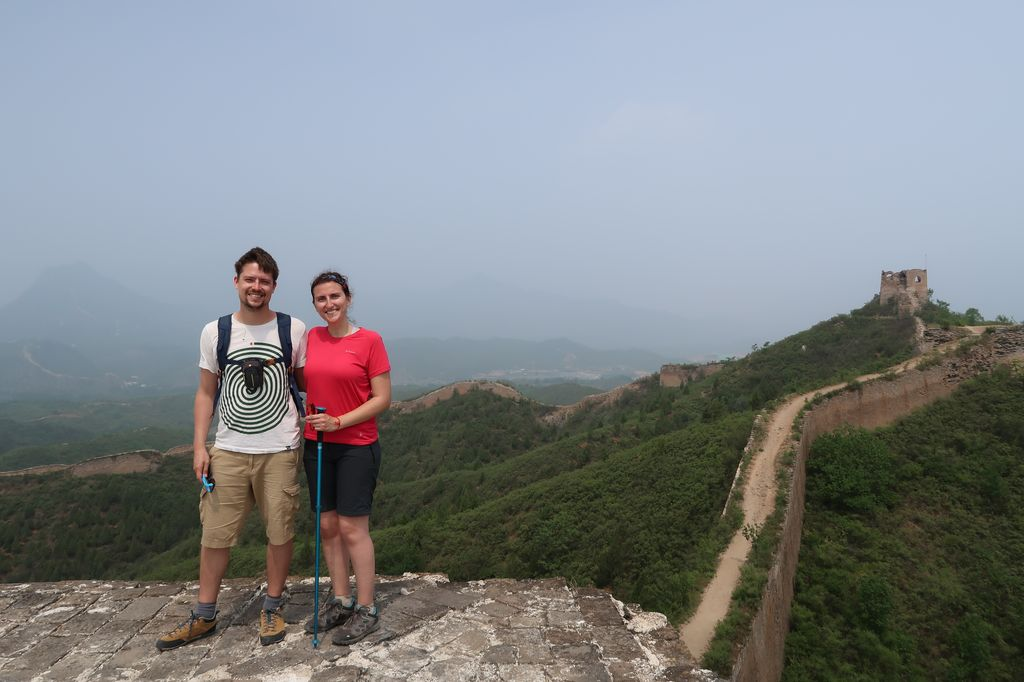
\includegraphics{images/20180616_muraille.JPG}
\caption{Debout sur la muraille de Chine, un moment dont on se
souviendra longtemps.}
\end{figure}

C'est avec un petit pincement au coeur qu'on quitte ce coin de
tranquilité pour notre deuxième train de nuit, direction Xi'an. Mais ça,
c'est pour la prochaine fois !

\emph{Elida et Florian}
